\subsection{Táblázatok}

%_
\begin{frame}
  \begin{columns}[c]
    \column{0.5\textwidth}
      Táblázatok alapértelmezett formázása:
      \begin{itemize}
        \item Cellaméretek a tartalomhoz igazodnak
        \item Nincsenek szegélyek
        \item Fejléc (\texttt{<th>}) cellák félkövérek, középre zártak
        \item Normál cellák (\texttt{<td>}) balra zártak
      \end{itemize}
    \column{0.45\textwidth}
        \begin{exampleblock}{\textattachfile{tablazat01.html}{tablazat01.html}}
          \begin{center}
            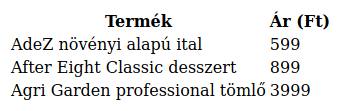
\includegraphics[width=\textwidth]{tablazat01.png}
          \end{center}
        \end{exampleblock}
  \end{columns}
\end{frame}

%_
\begin{frame}
  Kaphat szegélyt a teljes táblázat \dots
  \begin{columns}[c]
    \column{0.66\textwidth}
      \begin{exampleblock}{\textattachfile{tablazat02.html}{tablazat02.html}}
        \scriptsize
        \lstinputlisting[style=HTML,linerange={7-7},numbers=left,firstnumber=7]{tablazat02.html}
        \lstinputlisting[style=HTML,linerange={11-16},numbers=left,firstnumber=11]{tablazat02.html}
      \end{exampleblock}
    \column{0.3\textwidth}
      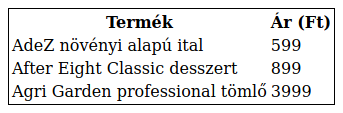
\includegraphics[width=\textwidth]{tablazat02.png}
  \end{columns}
\end{frame}

%_
\begin{frame}
  \dots vagy annak cellái \dots
  \vfill
  \begin{exampleblock}{\textattachfile{tablazat03.html}{tablazat03.html}}
    \lstinputlisting[style=HTML,linerange={7-7},numbers=left,firstnumber=7]{tablazat03.html}
  \end{exampleblock}
  \begin{center}
    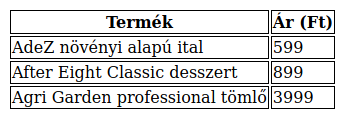
\includegraphics[width=0.4\textwidth]{tablazat03.png}
  \end{center}
\end{frame}

%_
\begin{frame}
  \dots vagy mindkettő.
  \vfill
  \begin{exampleblock}{\textattachfile{tablazat04.html}{tablazat04.html}}
    \lstinputlisting[style=HTML,linerange={7-7},numbers=left,firstnumber=7]{tablazat04.html}
  \end{exampleblock}
  \begin{center}
    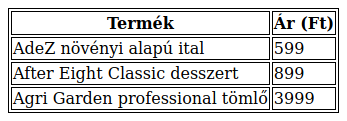
\includegraphics[width=0.4\textwidth]{tablazat04.png}
  \end{center}
\end{frame}

%_
\begin{frame}
  A cellák közötti távolság változtatható a \texttt{<table>} \texttt{border-spacing} tulajdonságával \dots
  \vfill
  \begin{exampleblock}{\textattachfile{tablazat05.html}{tablazat05.html}}
    \lstinputlisting[style=HTML,linerange={7-8},numbers=left,firstnumber=7]{tablazat05.html}
  \end{exampleblock}
  \begin{center}
    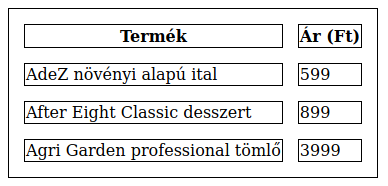
\includegraphics[width=0.4\textwidth]{tablazat05.png}
  \end{center}
\end{frame}

%_
\begin{frame}
  \dots de teljesen el is tüntethető a \texttt{<table>} \texttt{border-collapse} tulajdonságával:
  \begin{description}[m]
    \item[\texttt{separate}] elkülönített cellák, alapértelmezés.
    \item[\texttt{collapse}] összevont cellaszegélyek.
  \end{description}
  \vfill
  \begin{exampleblock}{\textattachfile{tablazat06.html}{tablazat06.html}}
    \lstinputlisting[style=HTML,linerange={7-8},numbers=left,firstnumber=7]{tablazat06.html}
  \end{exampleblock}
  \begin{center}
    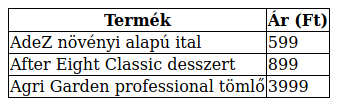
\includegraphics[width=0.4\textwidth]{tablazat06.png}
  \end{center}
\end{frame}

%_
\begin{frame}
  A cellák szegélye és tartalma közötti távolság a \texttt{<td>}, \texttt{<th>} \texttt{padding} tulajdonságával állítható.
  \begin{exampleblock}{\textattachfile{tablazat07.html}{tablazat07.html}}
    \footnotesize
    \lstinputlisting[style=HTML,linerange={7-11},numbers=left,firstnumber=7]{tablazat07.html}
  \end{exampleblock}
  \begin{center}
    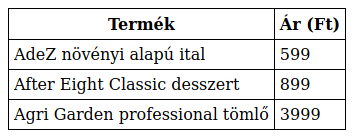
\includegraphics[width=0.4\textwidth]{tablazat07.png}
  \end{center}
\end{frame}

%_
\begin{frame}
  A cellákon belüli igazítás a \texttt{text-align}, \texttt{vertical-align} tulajdonságokkal állítható.
  \begin{exampleblock}{\textattachfile{tablazat08.html}{tablazat08.html}}
    \scriptsize
    \lstinputlisting[style=HTML,linerange={7-13},numbers=left,firstnumber=7]{tablazat08.html}
  \end{exampleblock}
  \begin{center}
    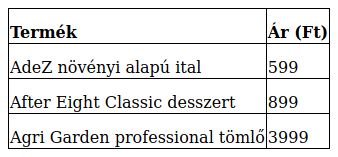
\includegraphics[width=0.35\textwidth]{tablazat08.png}
  \end{center}
\end{frame}

%_
\begin{frame}
  Ha a táblázat szélesebb, mint amit a tartalom indokol, a maradék hely arányosan lesz elosztva.
  \begin{exampleblock}{\textattachfile{tablazat09.html}{tablazat09.html}}
    \scriptsize
    \lstinputlisting[style=HTML,linerange={7-14},numbers=left,firstnumber=7]{tablazat09.html}
  \end{exampleblock}
  \begin{center}
    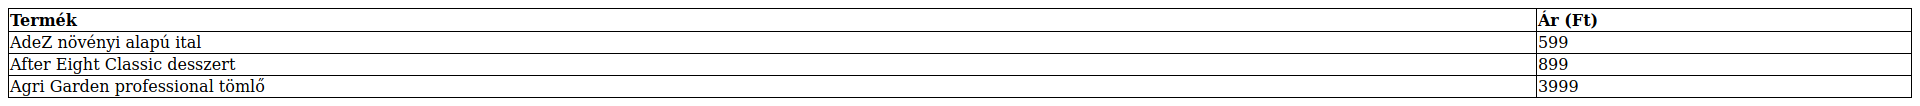
\includegraphics[width=\textwidth]{tablazat09.png}
  \end{center}
\end{frame}
